\documentclass[11pt]{article}

\usepackage{latexsym}
\usepackage{amsmath}
\usepackage{amssymb}
\usepackage{amsthm}
\usepackage{graphicx}
\usepackage{listings}
\graphicspath{ {./images/} }
\usepackage{wrapfig}
% \usepackage{pseudocode}
\usepackage{url}
\usepackage[backref, colorlinks=true, citecolor=red, urlcolor=blue, pdfauthor={Prakash Dhimal}]{hyperref}
\usepackage{chngcntr}
% does not reset figure counter.
\counterwithout{figure}{section}


\newcommand{\handout}[5]{
  \noindent
  \begin{center}
  \framebox{
    \vbox{
      \hbox to 5.78in { {\bf } \hfill #2 }
      \vspace{4mm}
      \hbox to 5.78in { {\Large \hfill #5  \hfill} }
      \vspace{2mm}
      \hbox to 5.78in { {\em #3 \hfill #4} }
    }
  }
  \end{center}
  \vspace*{4mm}
}

\newcommand{\lecture}[4]{\handout{#1}{#2}{#3}{#4}{#1}}

\newtheorem{theorem}{Theorem}
\newtheorem{corollary}[theorem]{Corollary}
\newtheorem{lemma}[theorem]{Lemma}
\newtheorem{observation}[theorem]{Observation}
\newtheorem{proposition}[theorem]{Proposition}
\newtheorem{definition}[theorem]{Definition}
\newtheorem{claim}[theorem]{Claim}
\newtheorem{fact}[theorem]{Fact}
\newtheorem{assumption}[theorem]{Assumption}

% 1-inch margins, from fullpage.sty by H.Partl, Version 2, Dec. 15, 1988.
\topmargin 0pt
\advance \topmargin by -\headheight
\advance \topmargin by -\headsep
\textheight 8.9in
\oddsidemargin 0pt
\evensidemargin \oddsidemargin
\marginparwidth 0.5in
\textwidth 6.5in

\parindent 0in
\parskip 1.5ex
%\renewcommand{\baselinestretch}{1.25}

\begin{document}

\lecture{Final Project Report: Visibility of Point Cloud}{Fall 2019}{Prakash Dhimal}{CS 633 Computational Geometry}

\begin{abstract}

Given a point cloud $ P = P_{1},P_{2},P_{3} ... P_{n} $ and a viewpoint $ C $, is it possible to determine all the points visible from $ C $ directly from the point cloud? Katz et al. \cite{Katz07} have shown that this is indeed the case and that this task can be performed without surface reconstruction and normal estimation. This paper investigates and implements an operator called the \textit{Hidden Points Removal} operator described in \cite{Katz07}, which computes only the visible points from a given viewpoint. The operator is simple and it consists of two steps:
\begin{enumerate}
\item Spherical inversion
\item Convex hull construction
\end{enumerate}

\paragraph{}
During Spherical inversion we transform the points to a new domain. Once the spherical inversion is performed, the convex hull of the transformed set of points union C, the viewpoint, is computed. Points that lie on the convex hull are visible from the given viewpoint.

\end{abstract}

\section{Motivation and Introduction}
We formally define a point cloud $ P $ as follows:
\begin{equation}
\label{eq:1}
P = P_{1},P_{2},P_{3} ... P_{n}
\end{equation}

A point cloud is simply a set of data points in space. It is a collection of points that represent a 3D shape or feature and might contain additional information about each point $ P_{i} $ such as color. Point clouds are most often created by remote sensing and 3D scanning devices such as Light Detection and Ranging (LiDAR). The use of LiDAR and similar 3D scanning devices have been increasing in the past decade. Figure \ref{simple-point-cloud} shows a simple point cloud with Red Green Blue values associated with each point $ P_{i} $. The simplicity of the point cloud data, the growing popularity of the 3D scanning devices as its sources, and its effectiveness and a powerful representation of all shapes and models have contributed to the popularity of point cloud data \cite{Mehra10}. 

Determining the visibility of point cloud is an interesting problem in itself. It is also useful in visualizing point clouds, in view-dependent reconstruction and in shadow casting \cite{Katz07}. Determining visibility can lead to a more robust registration of the points from multiple point clouds. This can also provide information about spatial relations and potential obstacles in the line of sight between two points in space, such analyses have been done in estimating the visibility of a landmark, and in finding the optimal location to place a surveillance camera.

\pagebreak
\begin{figure}[h]
	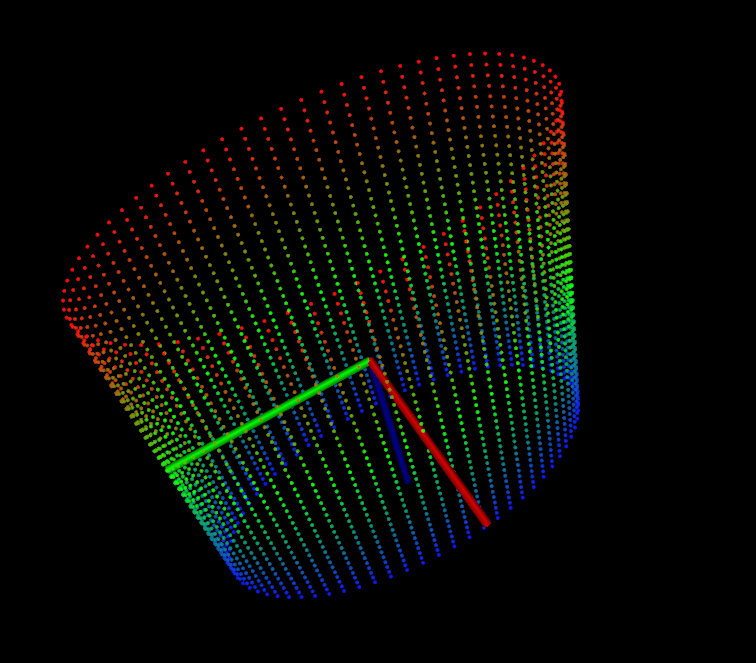
\includegraphics[width=7cm]{simple-pcl}
	\centering
	\caption{Sample Point Cloud}
	\label{simple-point-cloud}
\end{figure}

Suppose that we are given a point cloud depicting an object such as the bunny in figure \ref{fig:bunny-facing-which-way}. If all of the points are visualized, it is difficult to determine whether the bunny is facing forward or backward. After calculating all of the points visible from a given camera location it can be seen in figure \ref{fig:bunny-facing-front} that the bunny is facing forward.

\begin{figure}[h]
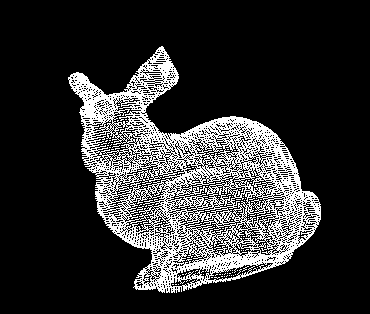
\includegraphics[width=7cm]{bunny-facing-which-way}
\centering
\caption{Is the Bunny facing forward or backward?}
\label{fig:bunny-facing-which-way}
\end{figure}


One way to compute the visibility of a point cloud is to reconstruct the surface and determine visibility on the reconstructed surface. Surface reconstruction is difficult and often requires additional information such as normals and only tends to work with the dense point cloud. In \cite{Katz07} it was shown that we can determine visibility without reconstructing a surface or estimating normals. This means that we can compute visibility directly from the point cloud. 

\begin{figure}[h]
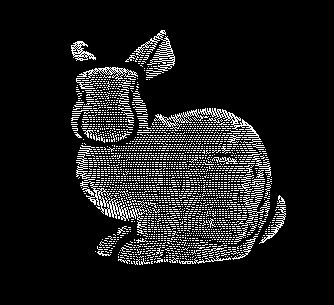
\includegraphics[width=7cm]{bunny-facing-front}
\centering
\caption{The Bunny is facing forward}
\label{fig:bunny-facing-front}
\end{figure}

\pagebreak
\section{Methods Used and Studied}

Given a Point cloud $ P = P_{1},P_{2},P_{3} ... P_{n} $, and a viewpoint \emph{C} our goal is to determine all of the points that are visible from $C $. To put it another way, for every point $ P_{i} $ in $ P$ we would like to determine if $ P_{i} $ is visible from $ C$. We would like to mark a point $ P_{i} $ visible if and only if the point $ P_{i} $ is visible from $ C$.

\subsection{Hidden Point Removal Operator}
Katz et al. \cite{Katz07} introduced an operator called the Hidden Point Removal operator that can be used to determine all of the points that are visible from $C$. The operator consists of two steps:

\begin{enumerate}
\item Spherical inversion
\item Convex hull construction
\end{enumerate}

During spherical inversion, we associate the points with a coordinate system where the viewpoint $C$ is at the origin. We then map every point $ P_{i} $ along the ray from $ C $ to $ P_{i} $ such that this mapping is monotonically decreasing in the norm ($ || P_{i} ||$). Once we perform the spherical inversion, we compute a convex hull of the transformed set of points $ union $ $ C$, the viewpoint. It is important to note that simply calculating the line of sight from the viewpoint $C$ to the point $ P_{i} $ will always mark the point as visible, except in some degenerate cases. 

What this operator is doing is a simple reduction of the problem of visibility to the problem of convex hull construction. This is because all we are doing is a simple transformation of the points and then computing the convex hull. The complexity of the operator is $ O(nlogn) $ in two and three dimensions and can be extended into higher dimensions. The complexity of the operator is asymptotically similar to that of convex hull construction, which is $ O(nlogn) $ in two and three dimensions.

\subsection{Spherical inversion}
Consider a D-dimensional sphere with radius $ R $, centered at the origin $ C $, and includes all points in P. Spherical inversion reflects a point $ P_{i} E P $ with respect to the sphere by applying the following equation: 

\begin{equation}
\label{eq:2}
f(P_{i}) = P_{i} + 2 (R - ||P_{i}||) \dfrac{P_{i}}{||P_{i}|} = \widehat{P_{i}}
\end{equation}

Spherical inversion is taking a point internal to some bounding sphere and projecting every point internal to the sphere to its image which is external to the using equation \ref{eq:2}. Spherical inversion reflects every point $ P_{i} $ internal to the sphere along the ray from $ C $ to $ P_{i} $ to its image outside the sphere, as shown in figure \ref{fig:spherical-inversion-1}. 

\begin{figure}[h]
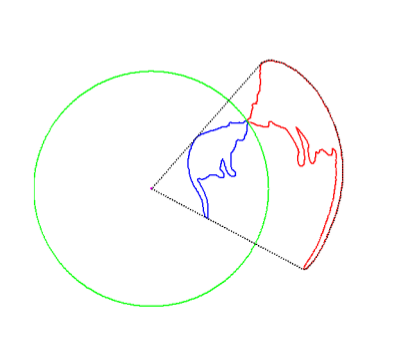
\includegraphics[width=7cm]{spherical-inversion-1}
\centering
\caption{Spherical inversion, shown in red, of a 2D curve, shown in blue, using a sphere, shown in green \cite{Katz07}}
\label{fig:spherical-inversion-1}
\end{figure}

Spherical inversion is taking the blue curve, which is constrained to be bounded in some green circle, which is centered at the origin, or the viewpoint $C$ in our case, and it maps the curve to its image that you see in red, which is the result of the spherical inversion.

\subsection{Convex Hull Construction}
From the spherical inversion above, we have a new point cloud that can be denoted as:
\begin{equation}
\label{eq:3}
\widehat{P} = \hat{P_{1}},\hat{P_{2}},\hat{P_{3}} ... \hat{P_{n}}
\end{equation}

The second, and the final step in our Hidden Point Removal operator is to construct the  convex hull of the new point cloud $\widehat{P} $ union $C$, i.e:

\begin{equation}
C_{hull} = \widehat{P} \cup C
\end{equation}

The points that lie on the convex hull $C_{hull}$ in the equation above are the points that are visible from $ C $. Figure \ref{fig:spherical-inversion-2} shows projection of the convex hull of the sphere in \ref{fig:spherical-inversion-1}.

\begin{figure}[h]
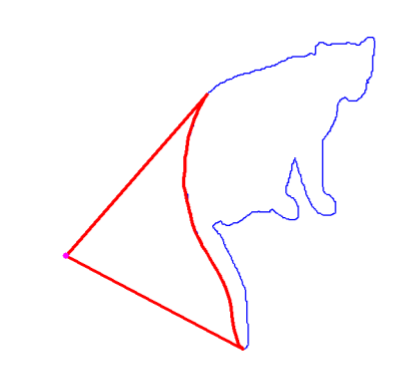
\includegraphics[width=7cm]{spherical-inversion-2}
\centering
\caption{Projection of the convex hull \cite{Katz07}}
\label{fig:spherical-inversion-2}
\end{figure}\textbf{•}

\subsection{The radius}
\label{section:radius}
An important drawback in Katz et al. \cite{Katz07} is that the discussion of the optimal radius is left out. In equation \ref{eq:2} the $ R $ is the radius of the inversion as shown in \ref{fig:spherical-inversion-1}. It was mentioned that a larger $ R $ relaxes the visibility condition and more points are considered visible. Thus, as $R$ increases, more points become visible, until all (truly visible) points become visible by the \textit{Hidden Point Removal} operator \cite{Katz07}.

One would jump to the conclusion that using an infinitely large radius would always produce the optimal results. But the authors also claimed that a large $R$ is suitable for dense point clouds, while a small $R$ is suitable for sparse clouds \cite{Katz07}. There is no one size fits all solution here. The readers are left on their own to figure out their own solution for the optimal radius. Mehra et al. \cite{Mehra10}, for example, came up with the optimal radius for noisy point clouds. The implementation of the Hidden Points Removal algorithm in this paper leaves the radius as an input to the algorithm, therefore it is left for the user to decide on the optimal radius based on their use cases. As shown in figure \ref{fig:point_cloud_library_with_HPR} users have the option to choose any radius they would like to compute visibility cloud with. 

\subsection{The data}
The initial plan was to use data obtained from the \textit{Velodyne HDL-64E LIDAR} scanner by the Motion and Shape Computing (MASC) Group at George Mason University to investigate the visibility of point clouds. While the Point Cloud Library (PCL) \cite{pcl} provides capabilities to read and replay/visualize such data, it became clear that determining visibility of a moving point cloud is beyond the scope of this project, as the implementation would need to support more complex data structures such as kinetic data structures to handle the moving point cloud. 

The data used in the scope of this project are all static models, such as the bunny from the Stanford 3D Scanning Repository. The statue of Michelangelo's David was obtained form the PCL's data repository. 

\section{Implementation and Results}

\subsection{The Hidden Point Removal operator implementation}
A simple MatLab code of the Hidden Point Removal operator was made publicly available by Katz et al. The goal was to implement this operator in C++ so that it can be used with the Point Cloud Library (PCL) for visualization and various other features that PCL provides. As such, the Hidden Point Operator (HPR) was implemented using PCL and various other libraries, such as Qt5, and VTK, in C++. The program  takes as an input a point cloud in \textit{PCD} or \textit{PLY} format. Figure \ref{fig:point_cloud_library_with_HPR} shows the program with a split window showing the original point cloud and the visibility cloud. This project, including the implementation, is also available at \href{https://github.com/pdhimal1/HPR.git}{https://github.com/pdhimal1/HPR.git}.

\begin{figure}[h]
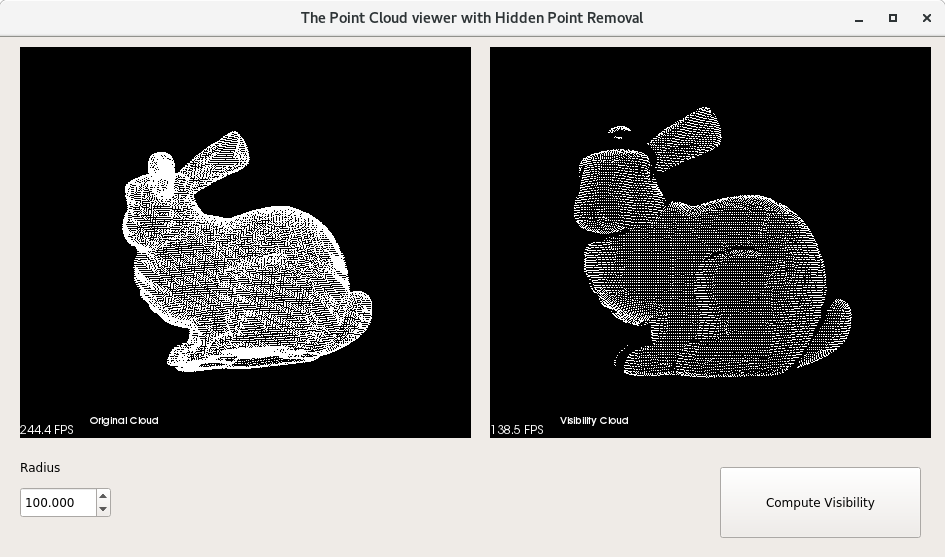
\includegraphics[width=12cm]{point_cloud_library_with_HPR}
\centering
\caption{The Point Cloud viewer with Hidden Point Removal}
\label{fig:point_cloud_library_with_HPR}
\end{figure}

As shown in figure \ref{fig:point_cloud_library_with_HPR}, a simple interface is provided to the user to calculate the visibility of a point cloud using the Hidden Point Removal operator. Two-point cloud viewers are provided to view the original point cloud and the visibility cloud side by side. As with any other point cloud viewers implemented using the Point cloud library, the user can change the viewpoint, or the camera location $C$, and move the point cloud around. When they are satisfied with the viewpoint, the user can also change the radius of the sphere $R$ as discussed in section \ref{section:radius}. Finally, the "Compute Visibility" button is provided for the user to click and compute all the points $\widehat{P} = \hat{P_{1}},\hat{P_{2}},\hat{P_{3}} ... \hat{P_{n}}$ that are visible from the camera location $C$ and the radius $R$ from the original point cloud $ P = P_{1},P_{2},P_{3} ... P_{n} $.

\subsection{Radius $R$ as an input}
As discussed in section \ref{section:radius}, the radius is an important input to the Hidden Point Removal operator. The implementation of the Hidden Point Removal operator in this project left the radius as an input to the operator, hence demanded a study of how the radius changes the result in the visibility cloud. Figure \ref{fig:Number-of-points-vs-radius} shows a chart in which the number of visible points increases as the radius increases.  

\begin{figure}[h]
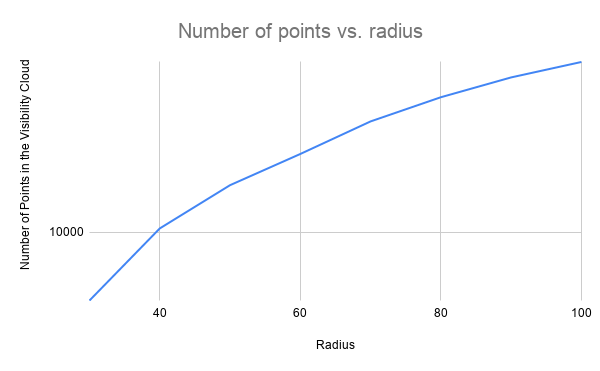
\includegraphics[width=12cm]{Number-of-points-vs-radius}
\centering
\caption{Number of points vs. radius}
\label{fig:Number-of-points-vs-radius}
\end{figure}

How does this affect the point clouds when they are visualized? Figure \ref{fig:bunny-looking-back-10} shows the output with $R$ as 10. As we can see, it looks like not all points that are visible from the camera location (on the original cloud frame) are visualized on the visibility cloud. Out of $35947$ points in the original point cloud, only $4597$ points are marked visible.


\begin{figure}[h]
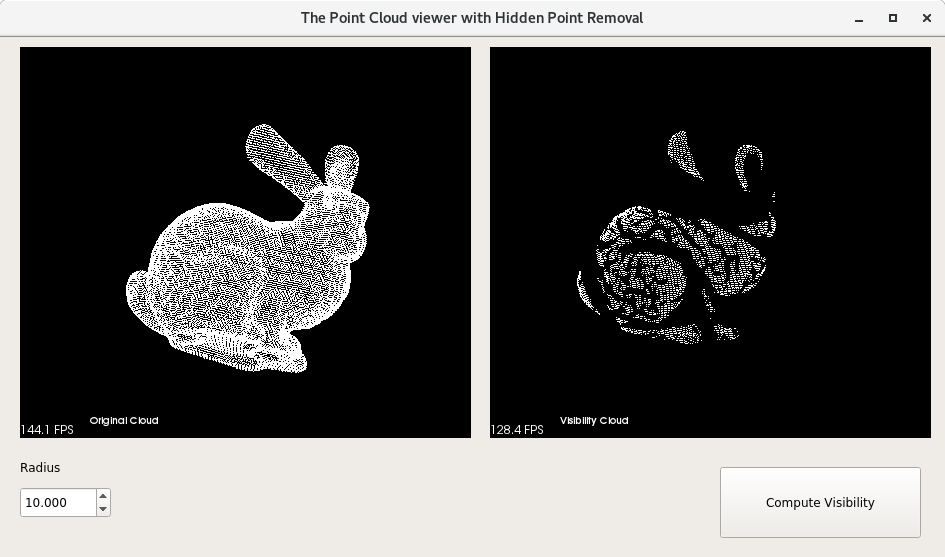
\includegraphics[width=12cm]{bunny-looking-back-10}
\centering
\caption{HPR with radius $R = 10$}
\label{fig:bunny-looking-back-10}
\end{figure}


Increasing the radius $R$ by five times, to $ R = 50 $, marks $10667$ as visible as shown in figure \ref{fig:bunny-looking-back-50}. It is important to mention that the camera location $C$ remained the same. Figure \ref{fig:bunny-looking-back-103} shows the result with $ R = 103 $. Here most of the points that are visible, to the human eye, on the original point cloud are marked visible and the result is satisfactory.

\begin{figure}[h]
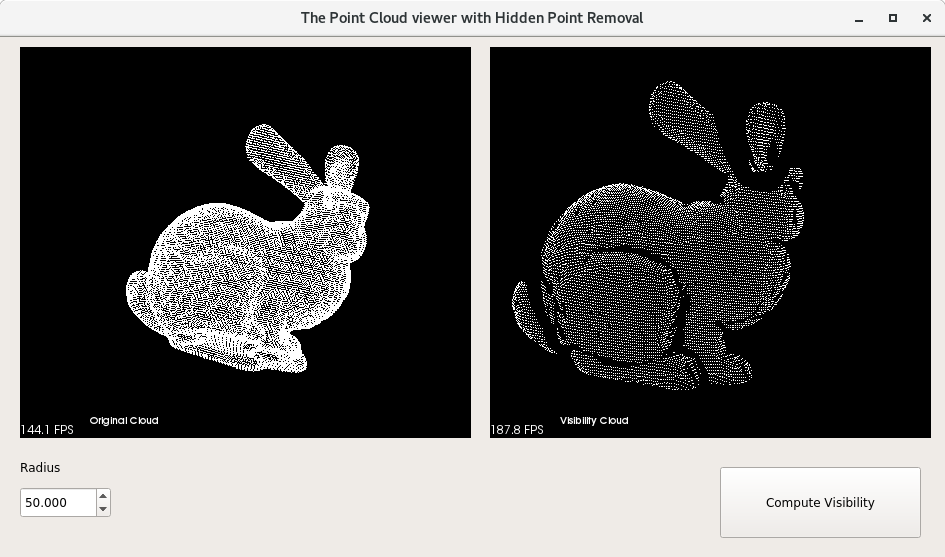
\includegraphics[width=12cm]{bunny-looking-back-50}
\centering
\caption{HPR with radius $R = 50$}
\label{fig:bunny-looking-back-50}
\end{figure}

\begin{figure}[h]
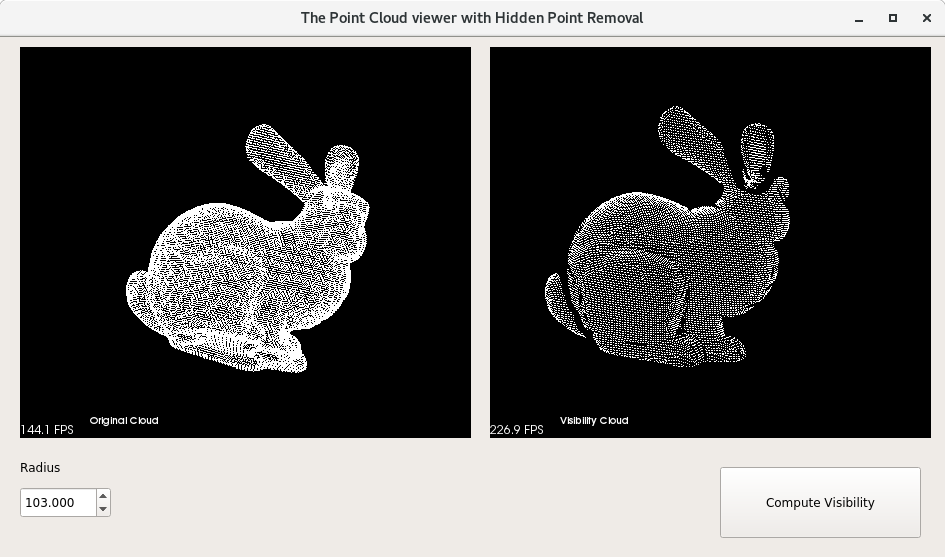
\includegraphics[width=12cm]{bunny-looking-back-103}
\centering
\caption{HPR with radius $R = 103$}
\label{fig:bunny-looking-back-103}
\end{figure}

\pagebreak

\section{Conclusion}
Given a point cloud $ P = P_{1},P_{2},P_{3} ... P_{n} $ and a viewpoint $ C $, it is possible to determine all the points visible from $ C $ \textbf{directly} from the point cloud. This work was inspired by Katz et al. \cite{Katz07} who first introduced the Hidden Point Removal operator in "Direct Visibility of Point Sets". The Hidden Point operator is easy to implement and works great to determine the visibility of a point cloud when used with the right selection of the radius $R$. As the point cloud data becomes more popular in the representation of shapes and models operators like this will be helpful not only to visualize the "visible points" but also to register point clouds from multiple sources. 

\nocite{Katz15}
\bibliographystyle{plain}
\bibliography{report}

\pagebreak
\begin{lstlisting}[language=matlab, caption=Matlab Implementation \cite{Katz07}]
function visiblePtInds=HPR(p,C,param)
	dim=size(p,2);
	numPts=size(p,1);
	% Move the points s.t. C is the origin
	p=p-repmat(C,[numPts 1]);
	% Calculate ||p||
	normp=sqrt(dot(p,p,2));
	% Sphere radius
	R=repmat(max(normp)*(10ˆparam),[numPts 1]);
	%Spherical flipping
	P=p+2*repmat(R-normp,[1 dim]).*p./repmat(normp,[1 dim]);
	%convex hull
	visiblePtInds=unique(convhulln([P;zeros(1,dim)]));
	visiblePtInds(visiblePtInds==numPts+1)=[];
\end{lstlisting}

\pagebreak

\begin{lstlisting}[language=c++, caption= C++ Implementation]
std::vector <pcl::visualization::Camera> cam;
viewer->getCameras(cam);
Eigen::Vector3d camera_location(
	cam[0].pos[0],
	cam[0].pos[1], 
	cam[0].pos[2]);
	
// ------ 1. Spherical Inversion -------------------
std::vector <Eigen::Vector3d> spherical_projection;
pcl::PointCloud<pcl::PointXYZ>::Ptr newCloud(
	new pcl::PointCloud <pcl::PointXYZ>);
for (size_t pidx = 0; pidx < cloud->points.size(); ++pidx) {
    pcl::PointXYZ currentPoint = cloud->points[pidx];
    Eigen::Vector3d currentVector(
    		currentPoint.x, currentPoint.y, currentPoint.z);
    Eigen::Vector3d projected_point = currentVector - camera_location;

    double norm = projected_point.norm();
    if (norm == 0)
        norm = 0.0001;

    // radius is set by the user using the radius editor
    // f(P_{i}) = P_{i} + 2 (R - ||P_{i}||) \dfrac{P_{i}}{||P_{i}|} = {P_{i}}
    spherical_projection.push_back(
        projected_point + 2 * (radius - norm) * projected_point / norm);
}

size_t origin_pidx = spherical_projection.size();
    
spherical_projection.push_back(Eigen::Vector3d(0, 0, 0));

for (std::size_t i = 0; i < spherical_projection.size(); ++i) {
    Eigen::Vector3d currentVector = spherical_projection.at(i);
    pcl::PointXYZ currentPoint(
    		currentVector.x(), currentVector.y(), currentVector.z());
    newCloud->push_back(currentPoint);
}
// ------ 2. Convex hull construction -------------------
pcl::PointCloud<pcl::PointXYZ>::Ptr cloud_hull(
	new pcl::PointCloud <pcl::PointXYZ>);
pcl::ConvexHull <pcl::PointXYZ> chull;
chull.setInputCloud(newCloud);
chull.reconstruct(*cloud_hull);

\end{lstlisting}

\listoffigures

\lstlistoflistings


%end of the document
\end{document}



